\documentclass[11pt]{article}

\usepackage{float}
\usepackage{hyperref}
\usepackage{fullpage}
\usepackage{verbatim}
\usepackage{moreverb}
\usepackage{graphicx}
\usepackage{parskip}
\usepackage[toc,page]{appendix}

\usepackage{minted}
\let\verbatiminput=\verbatimtabinput
\def\verbatimtabsize{4\relax}

\begin{document}
\title{EE 241B HW1 Writeup}

\author{Vighnesh Iyer}
\date{}
\maketitle

\tableofcontents

\section{Models - MOSFET Characterization}

We are using a 32nm LP CMOS process for this class. The devices being characterized are \verb|n105| and \verb|p105| (TT corner) with a nominal supply voltage of 1.05V.

\subsection{Threshold Voltages}
We want to determine the threshold voltage $V_{th}$ for the NMOS and PMOS devices (for $V_{BS}$ = 0, $L$ = 32nm, and $W$ = 1$\mu$m), by extrapolating from the $I_DS$ vs. $V_{GS}$ curve at low $V_{DS}$. We compare the threshold voltage derived from DC sweeps to the values reported in the model file and the DC operating point analysis.

To perform this characterization, we first collect a full range of DC operating points for both transistors to make analysis easier for this entire section. The transistors' drains are connected to a variable DC supply and the transistors' gates are connected to another independent variable DC supply. The source for both transistors is held at ground (0V). We perform a nested DC analysis by sweeping $V_{DS}$ from $0 \rightarrow 1.05$V in (10mV) increments, and sweep $V_{GS}$ from $0 \rightarrow 1.05$V in (10mV) increments.

The gathered I-V curves are shown below.

\begin{figure}[H]
	\centerline{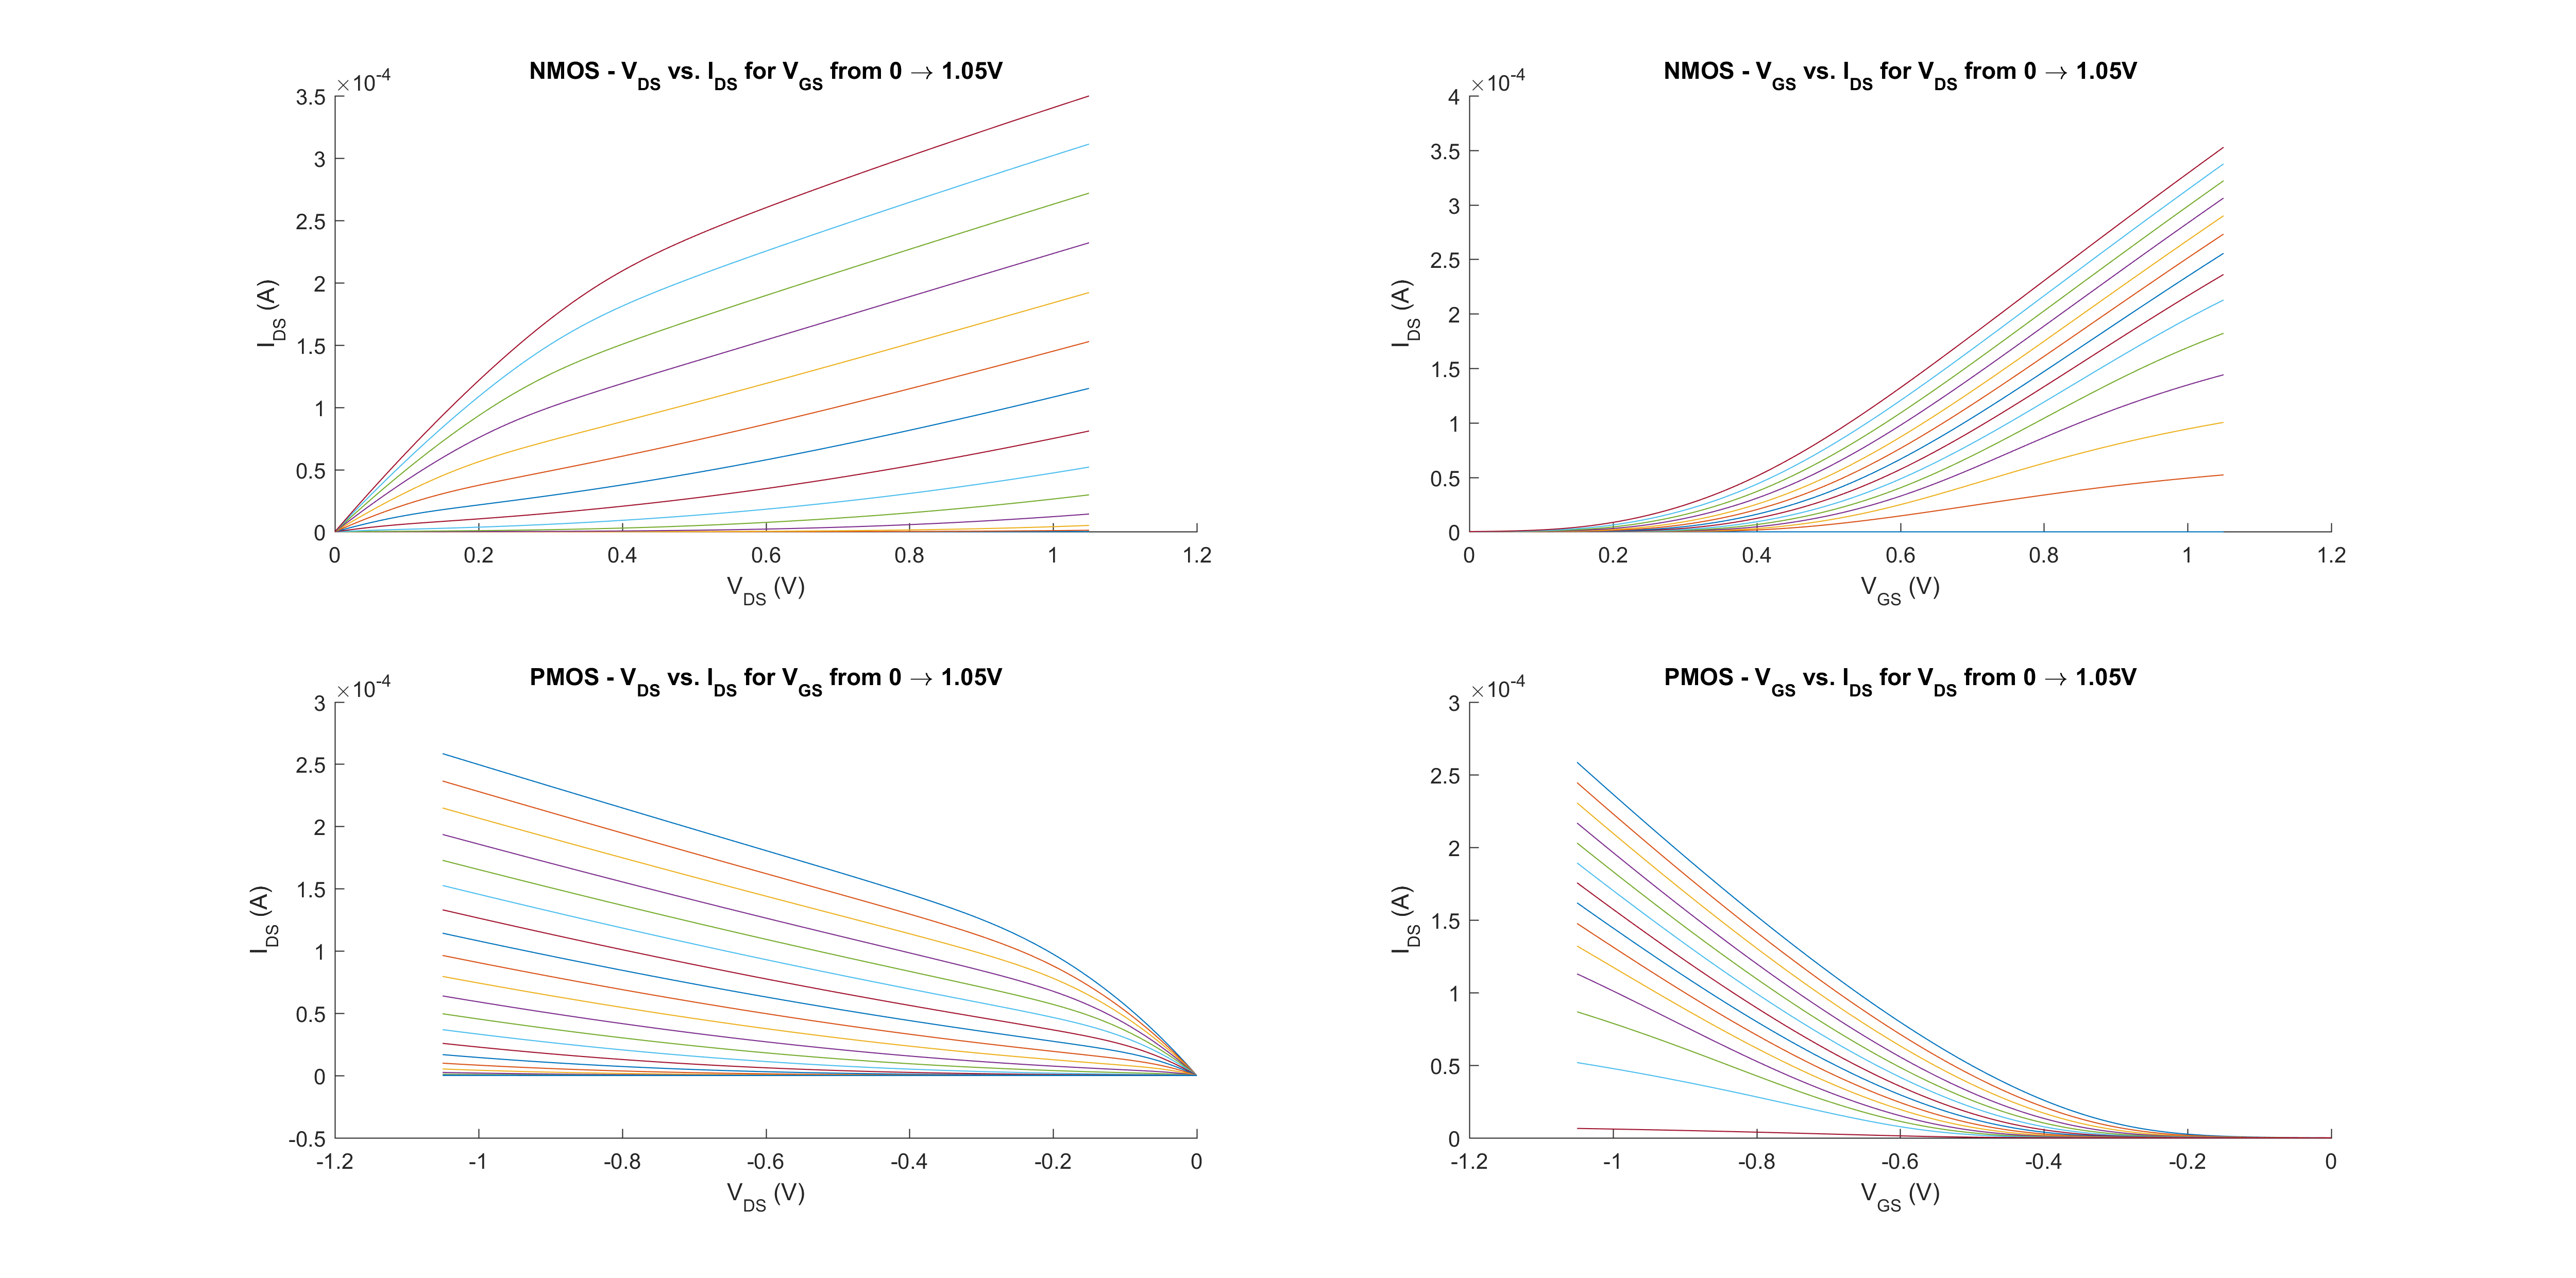
\includegraphics[width=\textwidth+5cm]{images/dc_curves.png}}	
\end{figure}

From the DC OP analysis, $V_{th}$ of the NMOS is reported to be 324.4 mV, and the $V_{th}$ of the PMOS is reported to be -208.1 mV. From the model files the NMOS $V_{th}$ is 370 mV, and the PMOS $V_{th}$ is -213 mV.

To extract the threshold voltage from 

\newpage
\appendix
\section{PMOS/NMOS DC Characterization SPICE Sim} \label{dc_characterization_spice}
\begin{minted}{text}
Sweep of V_GS with constant V_DS for N-MOSFET
.lib '/home/ff/ee241/synopsys-32nm/hspice/saed32nm.lib' TT
vds vds gnd 1.05
vgs vgs gnd 1.05 
x1 vds vgs gnd gnd n105 (w=1u l=32n)

.op
.dc vgs 0 1.05 10m vds 0 1.05 10m

.option post=2 nomod
.end
\end{minted}

\section{}

\end{document}